\subsection{同胚群上的拓扑}

命题 10. 设 X 是一致空间，H 是 X 到其自身上的同胚所成的一个等度连续集。若 H 与 \(H^{-1}\) 都赋有 X 中逐点收敛的拓扑，则映射 \(u \rightarrow u^{-1}\) （由 \(H^{-1}\) 到 H 上）是连续的。

只需证明，对每个 \(x_0 \in \mathbf{X}\) ，映射 \(u \to u^{-1}(x_0)\) （由 \(\mathbf{H}^{-1}\) 到 \(\mathbf{X}\) 中）在每一点 \(u_0 \in \mathbf{H}^{-1}\) 处连续。设 \(\mathbf{V}\) 是 \(\mathbf{X}\) 的一个对称围域，并设 \(y_0 = u_0^{-1}(x_0)\) 。由假设，存在对称围域 \(\mathbf{U}\) （\(\mathbf{X}\) 的围域），使得关系 \((x, x_0) \in \mathbf{U}\) 蕴涵 \((u^{-1}(x), u^{-1}(x_0)) \in \mathbf{V}\) 对一切 \(u \in \mathbf{H}^{-1}\) 成立。取一个元素 \(u \in \mathbf{H}^{-1}\) ，它是 \(W(\{y_0\}, \mathbf{U})\) -接近于 \(u_0\) 的；则我们有 \((u(y_0), u_0(y_0)) \in \mathbf{U}\) ，即 \((u(y_0), x_0) \in \mathbf{U}\) 。由此得出 \((y_0, u^{-1}(x_0)) \in \mathbf{V}\) ，即 \((u_0^{-1}(x_0), u^{-1}(x_0)) \in \mathbf{V}\) ；证明完成。

推论. 设 X 是一致空间，H 是 X 到其自身上的同胚所成的一个等度连续群。则 X 中逐点收敛的拓扑与 H 的群结构相容。

这是命题 10 连同第 2 节第 1 号命题 1 的推论 5 的推论。

命题 11. 设 X 是紧空间，\(\Gamma\) 是 X 到其自身上的一切同胚所成的群。则 X 中的一致收敛拓扑与 \(\Gamma\) 的群结构相容。

我们已经知道（第 4 号，命题 9）映射 \((u, v) \to v \circ u\) （由 \(\Gamma \times \Gamma\) 到 \(\Gamma\) 中）关于这个拓扑连续；于是只需证明 \(u \to u^{-1}\) 在每一点 \(u_0\) （\(\Gamma\) 的点）处连续。由于 \(u_0^{-1}\) 在 \(\mathbf{X}\) 上一致连续，对任一对称围域 \(\mathbf{V}\) （\(\mathbf{X}\) 的围域），存在一个围域 \(\mathbf{W}\) （\(\mathbf{X}\) 的围域），使得关系 \((x, x') \in \mathbf{W}\) 蕴涵 \((u_0^{-1}(x), u_0^{-1}(x')) \in \mathbf{V}\) 。因此，若 \(u \in \Gamma\) 使 \((u_0(x), u(x)) \in \mathbf{W}\) 对一切 \(x \in \mathbf{X}\) 成立，则得出 \((x, u_0^{-1}(u(x))) \in \mathbf{V}\) 对一切 \(x \in \mathbf{X}\) 成立，从而（由于 \(u\) 是双射）\((u^{-1}(x), u_0^{-1}(x)) \in \mathbf{V}\) 对一切 \(x \in \mathbf{X}\) 成立。证明完成。

\pandocbounded{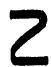
\includegraphics[keepaspectratio]{images/part002_d26bd6ea.jpg}}

现在设 X 是局部紧空间，\(\Gamma\) 是 X 到其自身上的一切同胚所成的群。X 中紧收敛的拓扑不必与 \(\Gamma\) 的群结构相容（习题 17）。用 \(X'\) 表示由 X 添加一个无穷远点 \(\omega\) 所得到的紧空间。X 到其自身上的每个同胚 u 都唯一扩张为一个同胚 \(u'\) （\(X'\) 到其自身上的），使 \(u'(\omega) = \omega\) （第 I 章，§ 10，第 3 号，命题 7 的推论），于是 \(\Gamma\) 可等同于 \(\Gamma'\) （\(X'\) 到其自身上的一切同胚所成的群）中由使 \(\omega\) 不动的一切同胚组成的子群。因此 \(\Gamma\) 上由 \(C_u(X'; X')\) 的拓扑诱导的拓扑与 \(\Gamma\) 的群结构相容（命题 11），且 \(\Gamma\) 在 \(\Gamma'\) 中是闭的{[}关于由 \(\mathcal{C}_u(\mathbf{X}';\mathbf{X}')\) 的拓扑诱导的拓扑{]}，因为它由方程 \(u(\omega)=\omega\) 定义（\(\S\) 1，第 2 号，注 6）。我们用 \(\mathcal{C}_{\beta}\) 表示这样定义在 \(\Gamma\) 上的群拓扑；它比紧收敛的拓扑细，并且也可（借助 \(\S\) 1，第 6 号，命题 6）定义为 \(\mathbf{X}\) 上一致收敛的拓扑，当 \(\mathbf{X}\) 赋有由 \(\mathbf{X}'\) 的唯一一致结构诱导的一致结构时。

拓扑 \(\mathcal{C}_{\beta}\) 可刻画如下：

命题 12. 在群 \(\Gamma\) （局部紧空间 \(\mathbf{X}\) 的一切同胚所成的群）上，拓扑 \(\mathcal{C}_{\beta}\) 是使映射 \(u \to u\) 与 \(u \to u^{-1}\) （由 \(\Gamma\) 到 \(\mathcal{C}_c(\mathbf{X}; \mathbf{X})\) 中）连续的最粗拓扑。

暂把这个拓扑记作 \(\mathcal{C}'\) 。由于 \(u \to u^{-1}\) 关于 \(\mathcal{C}_{\beta}\) 连续，且 \(\mathcal{C}_{\beta}\) 比紧收敛的拓扑细，显然 \(\mathcal{C}_{\beta}\) 比 \(\mathcal{C}'\) 细。为证明其逆，给 \(\mathbf{X}'\) 赋予它的唯一一致结构；设 \(u_0 \in \Gamma\) ，并设 \(\mathbf{V}\) 是 \(\mathbf{X}'\) 的一个围域；于是我们必须证明存在一个紧子集 \(\mathbf{K}\) （\(\mathbf{X}\) 的）与一个对称围域 \(\mathbf{W}\) （\(\mathbf{X}'\) 的），使得关系

\[
u \in \Gamma , (u _ {0} (x), u (x)) \in \mathrm{W} \text {   and   } (u _ {0} ^ {- 1} (x), u ^ {- 1} (x)) \in \mathrm{W} \text {   for   all   } x \in \mathrm{K}
\]

蕴涵

\[
(u _ {0} (x), u (x)) \in \mathbf {V} \text {   for   all   } x \in \mathbf {X}.
\]

设 \(V_1\) 是 \(X'\) 的一个对称开围域，使 \(\dot{V}_1 \subset V\) ；则 \(K_1 = X' - V_1(\omega)\) 是 \(X\) 的一个紧子集。选取一个对称开围域 \(W\) （\(X'\) 的），使 \(W \subset V\) 且 \(W(\omega) \cap W(u_0^{-1}(K_1)) = \emptyset\) ；由第 II 章，§ 4，第 3 号，命题 4，这是可能的。设 \(K_2 = X' - W(\omega)\) ，它是 \(X\) 的一个紧子集。我们将看到 \(W\) 与紧集 \(K = K_1 \cup K_2\) 满足要求。由于 \(W \subset V\) ，只需证明关系

\[
\left(u _ {0} ^ {- 1} (x), u ^ {- 1} (x)\right) \in \mathrm{W} \quad \text { for   all } \quad x \in \mathrm{K} _ {1} \quad (u \in \Gamma)
\]

蕴涵

\[
(u (y), \omega) \in \mathrm{V} _ {1} \quad \text { for   all } \quad y \in \mathrm{W} (\omega);
\]

因为那时我们也将有 \((u_0(y),\omega)\in \mathbf{V}_1\) ，从而

\[
(u _ {0} (y), u (y)) \in \mathring {\mathrm{V}} _ {1} ^ {2} \subset \mathrm{V}
\]

对一切 \(y \in W(\omega) = X' - K_2\) 。现在，若我们有 \(y \in W(\omega)\) 且

\[
u (y) \in \mathrm{X} ^ {\prime} - \mathrm{V} _ {1} (\omega) = \mathrm{K} _ {1},
\]

则将得出 \(y \in u^{-1}(\mathbf{K}_1) \subset W(u_0^{-1}(\mathbf{K}_1))\) ，与 \(W\) 的选取相矛盾；因此证明完成。

一般地，群 \(\Gamma\) （赋有 \(\mathfrak{G}_{\beta}\) ）不是局部紧的；但我们有如下的判别法：

定理 4. 设 G 是局部紧空间 X 的一切同胚所成的群 \(\Gamma\) 的一个子群。假设在空间 \(\mathcal{C}_{\mathfrak{c}}(\mathbf{X};\mathbf{X})\) 中有恒等映射 \(e\) 的一个邻域 V 使 \(\mathbf{V}\cap \mathbf{G} = \mathbf{H}\) 在 G 中对称且在 \(\mathcal{C}_{\mathfrak{c}}(\mathbf{X};\mathbf{X})\) 中相对紧。则闭包 \(\overline{\mathbf{G}}\) （G 在 \(\Gamma\) 中关于拓扑 \(\mathcal{T}_{\beta}\) 的闭包）关于由 \(\mathcal{T}_{\beta}\) 诱导的拓扑是一个局部紧群；在 \(\overline{\mathbf{G}}\) 上诱导的这个拓扑与紧收敛的拓扑相同，且闭包 \(\overline{\mathbf{H}}\) （H 在 \(\mathcal{C}_{\mathfrak{c}}(\mathbf{X};\mathbf{X})\) 中的闭包）是 \(e\) 在 \(\overline{\mathbf{G}}\) 中关于这个拓扑的一个邻域。

首先证明 \(\overline{\mathbf{H}}\) 含于 \(\Gamma\) ，且 \(\overline{\mathbf{H}}\) 上由 \(\mathfrak{C}_{\beta}\) 诱导的拓扑与紧收敛的拓扑相同。设 \(u_0 \in \overline{\mathbf{H}}\) ；于是 \(u_0\) 在 \(\mathcal{C}_c(\mathbf{X}; \mathbf{X})\) 中是超滤子 \(\Phi\) （在 \(\mathbf{H}\) 上）的极限。由于 \(\Phi^{-1}\) （\(\Phi\) 在映射 \(u \to u^{-1}\) 下的像）是 \(\mathbf{H} \subset \overline{\mathbf{H}}\) 上的一个超滤子基，它在紧子空间 \(\overline{\mathbf{H}}\) （\(\mathcal{C}_c(\mathbf{X}; \mathbf{X})\) 的子空间）中收敛于一个元素 \(v_0\) 。映射 \((u, v) \to uv\) 收敛于 \(u_0 v_0\) （关于 \(\Phi \times \Phi^{-1}\) ）（第 4 号，命题 9）；更有甚者，\(u \to uu^{-1} = e\) 收敛于 \(u_0 v_0\) （关于 \(\Phi\) ），故 \(u_0 v_0 = e\) ，因为 \(\mathcal{C}_c(\mathbf{X}; \mathbf{X})\) 豪斯多夫。同样 \(v_0 u_0 = e\) ；于是 \(u_0\) 是 \(\mathbf{X}\) 的一个同胚，即 \(u_0 \in \Gamma\) 。这样 \(\overline{\mathbf{H}}\) 含于 \(\Gamma\) 。此外，这个论证表明 \(\overline{\mathbf{H}}^{-1} = \overline{\mathbf{H}}\) ，且对每个超滤子 \(\Phi\) （在 \(\overline{\mathbf{H}}\) 上，收敛于 \(u_0\) ），\(\Phi^{-1}\) 在 \(\mathcal{C}_c(\mathbf{X}; \mathbf{X})\) 中收敛于 \(u_0^{-1}\) ；因此映射 \(u \to u^{-1}\) （由 \(\overline{\mathbf{H}}\) 到 \(\mathcal{C}_c(\mathbf{X}; \mathbf{X})\) 中）当 \(\overline{\mathbf{H}}\) 带有紧收敛的拓扑时连续（第 I 章，§ 7，第 4 号，命题 9 的推论 1）。于是命题 12 表明，在 \(\overline{\mathbf{H}}\) 上，紧收敛的拓扑与由 \(\mathfrak{C}_{\beta}\) 诱导的拓扑相同。

此外，由于拓扑 \(\mathcal{C}_{\beta}\) （在 \(\Gamma\) 上）比紧收敛的拓扑细，\(\overline{\mathbf{H}}\) 也是 \(\mathbf{H}\) 关于 \(\mathcal{C}_{\beta}\) 的闭包。但 \(\mathbf{H}\) 是 \(e\) 在 \(\mathbf{G}\) 中关于紧收敛的拓扑的一个邻域，从而更是关于由 \(\mathcal{C}_{\beta}\) 诱导的拓扑的邻域；由此（第 I 章，§ 3，第 1 号，命题 2）得出，\(\overline{\mathbf{H}}\) 是 \(e\) 在 \(\overline{\mathbf{G}}\) 中关于由 \(\mathcal{C}_{\beta}\) 诱导的拓扑的一个邻域，因此 \(\overline{\mathbf{G}}\) 关于这个拓扑是局部紧的。若 \(\mathbf{W}\) 是 \(\mathbf{V}\) 关于紧收敛的拓扑的内部，则 \(\mathbf{W} \cap \Gamma\) 在 \(\mathcal{C}_{\beta}\) 中开，因此 \(\mathbf{W} \cap \overline{\mathbf{G}}\) 含于 \(\mathbf{H} = \mathbf{V} \cap \mathbf{G}\) 关于 \(\mathcal{C}_{\beta}\) 的闭包（第 I 章，§ 1，第 6 号，命题 5）；这表明 \(\overline{\mathbf{H}}\) 也是 \(e\) 在 \(\overline{\mathbf{G}}\) 中关于紧收敛的拓扑的一个邻域。最后，对每个 \(u_{0} \in \Gamma\) ，双射 \(v \to u_{0} \circ v\) 与 \(v \to u_{0}^{-1} \circ v\) （由 \(\mathcal{C}_{c}(\mathbf{X}; \mathbf{X})\) 到其自身上）连续（第 4 号，命题 9），因此，若 \(u_{0} \in \overline{G}\) ，则 \(u_{0}\overline{H}\) 是 \(u_{0}\) 在 \(\overline{G}\) 中关于紧收敛的拓扑的一个邻域。证明完成。

推论. 设 G 是局部紧空间 X 的一个同胚群。若闭包 \(\overline{G}\) （G 在 \(\mathcal{C}_{c}(X; X)\) 中的闭包）紧，则 \(\overline{G}\) 是 X 的一个同胚群，且紧收敛的拓扑与 \(\overline{G}\) 的群结构相容，因而它是一个紧拓扑群。

\pandocbounded{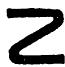
\includegraphics[keepaspectratio]{images/part002_e2b18e11.jpg}}

局部紧空间 X 的一个同胚群，若关于紧收敛的拓扑局部紧但不紧，则由第 I 章，§ 9，第 7 号，命题 12，它在 \(\mathcal{C}_{c}(\mathbf{X};\mathbf{X})\) 中是局部闭的，但不必是闭的。

例如，在环 \(\mathcal{L}(\mathbf{R}^{n})\) （\(\mathbf{R}^{n}\) 的自同态所成的环）中——这个环等同于方阵环 \(\mathbf{M}_{n}(\mathbf{R})\) （\(n \times n\) 方阵，在 \(\mathbf{R}\) 上）且赋有紧收敛的拓扑——，群 \(\mathbf{GL}(n, \mathbf{R})\) （等同于非奇异矩阵所成的群）局部紧但稠密（第 VI 章，§ 1，第 6 号，命题 6）。

